% !TEX root = ../main.tex

% open questions section

\section{Quantifying the Distance between MLE to its Asymptotic Distribution}
To describe the distance between two distributions, or two random variables following two different distributions, a \emph{Zolotarev-type distance}, as defined in \cite{zolotarev1976metric}, can be used, as it is a natural extension of a metric from non-probabilistic spaces to probabilistic ones. One of the simplist of such distances is
\begin{align}
D(X,Y) = \sup_{h\in H} \left| \bbE\left[h(X)\right] - \bbE\left[h(X)\right] \right|, && H \text{ is the set of continous and bounded real functions},
\end{align}
for it satisfies the following probabilistic versions of properties of a metric:
\begin{itemize}
\item $\bbP(X=Y) \implies D(X,Y) = 0$,
\item $D(X,Y) = D(Y,X)$,
\item $D(X,Y) \leq D(X,Z) + D(Z,Y)$, for $Z\neq X, Z\neq Y$.
\end{itemize}
By \cref{thm:1}, we have that $\sqrt{nI(\theta_0)}(\hat{\theta} - \theta_0) \convD \calN(0, 1)$. Then with $Y = \sqrt{nI(\theta_0)}(\hat{\theta} - \theta_0)$ and $Z=\calN(0,1)$, $D(Y,Z)$ describes the closeness from the MLE approximated using finitely many observations to the asymptotic normal distribution. \cite{anastasiou2015bounds} developed a bound on exactly the quantity $D(Y,Z)$ in the one-dimensional case, for random variables $X$ where there exists a one-to-one twice differentiable mapping $q: \Theta \rightarrow \bbR$ such that $q(\hat{\theta})=\sum_{i=1}^n g(X_i)$ for some $g:\bbR\rightarrow\bbR$. The main theorem is presented below.
\begin{theorem}\label{thm:3}
Under regularity conditions and following the notations set up in \cref{sec:notation} and the beginning of this section, let $q:\Theta \rightarrow \bbR$ be a one-to-one twice differentiable function with $q'(\theta) \neq 0 \forall \theta\in\Theta$ and such that $q\left( \hat{\theta}_n(\bm{X})\right) = \frac{1}{n}\sum_{i=1}^n g(X_i)$, where the mapping $g:\bbR\rightarrow\bbR$ is such that $\bbE\left[ \left| g(X_1)-q(\theta_0) \right|^3 \right] < \infty$ for the true parameter $\theta_0$. Also, there exists a positive constant $0 < \epsilon = \epsilon(\theta_0)$ with $(\theta_0 - \epsilon, \theta_0 + \epsilon) \subset \Theta$.Then for any $h\in H$, we have
\begin{align*}
&\left| \bbE\left[ h\left(\sqrt{nI(\theta_0)}(\hat{\theta} - \theta_0)\right) \right] - \bbE\left[h(Z)\right] \right|\\
&\leq \frac{\|h'\|_\infty}{\sqrt{n}}\left(2 + \frac{\left[I(\theta_0)\right]^{3/2}}{|q'(\theta_0)|^3} \bbE\left[\left|g(X_1) - q(\theta_0)\right|^3\right] \right) \\
&+\bbE\left[(\hat{\theta}(\bm{X})-\theta_0)^2\right]\left( 2\frac{\|h\|_\infty}{\epsilon^2}\mathbf{1}\{\exists\theta\in\Theta:q(\theta)\neq\theta\}+\frac{\|h'\|_\infty\sqrt{nI(\theta_0)}}{2|q'(\theta_0)|}\text{sup}_{\theta:|\theta-\theta_0|\leq\epsilon}|q''(\theta)| \right).
\end{align*}
\end{theorem}$ $\\
Note that for any $h\in H$, the above bound gives a lowerbound of $D(X,Y)$, since \emph{Zolotarev-type distances} take the supremum over all such functions. Compared to \cref{thm:1,thm:2}, the above result provides a quantitative measure on the distance between the unknown distribution of MLE based on finitely many observations and its corresponding asymptotic distribution. The proof of \cref{thm:3} is similar to that of \cref{thm:1} in that they both start with obtaining an expression of the quantity of interest followed by analysis of each of the terms in the expression. In this particular case, the triangle inequality is first applied on $D(Y,Z)$, and each of the two terms can then be bounded using a combination of the delta method, Stein's method, and Taylor expansions.\\\\
To verify the above theorem, we perform another set of simulations, comparing the bound on the MLE of Gamma$(\alpha=2,\theta=2)$ given $\alpha$. In particular, we generate $10000$ trials of $n=10,100,1000,10000,100000$ \iid observations from Gamma$(\alpha=2,\theta=2)$, using the shape and scale parameterization. With the choice of $h(x)=\frac{1}{x^2+2}$, we have $\|h\|_\infty = 0.5, \|h'\|_\infty = 3\sqrt{1.5}/16, \bbE\left[h(Z)\right] = 0.379$. Then we can compute a Monte-Carlo approximation of $D(Y,Z)$ by averaging over all $10000$ trials of $h\left(\sqrt{nI(\theta_0)}(\hat{\theta} - \theta_0)\right)$. This is then compared to the bound in \cref{thm:3}, under the more specific case as laid out in Section 3.2 of \cite{anastasiou2015bounds}. (\cref{simulation}). The code can be found at \texttt{src/simulation\_bound.R}. \texttt{RStudio 1.3.959} is used to generate the plots below.\\\\
Note that since there is only one parameter to be estimated, the MLEs are very close to the true value even with a not-so-large sample size, and so the black line on the plot may not always be monotonically decreasing. We do note, however, that the bound developed in \cref{thm:3} becomes tighter as the sample size increases.
\begin{figure}[h]
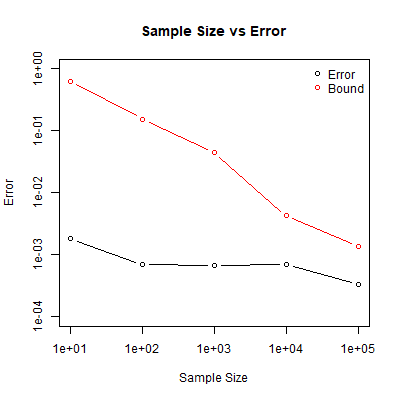
\includegraphics[scale=0.4]{../../../misc/rplot.jpg}
\centering
\caption{Sample size vs. Zolotarev distance}
\label{simulation}
\end{figure}$ $\\
There are many directions of future research on the topic. As an example, it would be interesting to see if we can transform the bound in \cref{thm:3} to some inequalities on the approximate confidence intervals of $\theta_0$, either deterministically or probabilistically. As another example, we note that \cite{anastasiou2015bounds} only discussed the one-dimensional case, and as seen in both of our simulations, the MLE gets quite close to its asymptotic distribution even with a not-so-large sample size. It would be a natural next step to extend the bound in \cref{thm:3} to multi-dimensional settings. We offer some initial ideas on this extension.\\\\
Glancing through the proof in \cite{anastasiou2015bounds}, many of the results applied in the process of achieving the final result has multivariate versions. Particularly, all of the triangle inequality, delta method, and Taylor expansions can be applied directly in the multivariate setting. The bottleneck then becomes developing multivariate versions of two of the lemmas used in the proof. Namely, Lemma 2.1 in \cite{anastasiou2015bounds} and Lemma 2.1 in \cite{anastasiou2017bounds}.